%% Appendix

\section{Data Construction Details}
\label{asec:data_construction}

\subsection{VIIRS Nighttime Lights}
\label{asec:viirs_construction}

The monthly \VIIRS{} composites were extracted via Google Earth Engine
using the VNP46A3.001 product (NASA Black Marble Monthly). For each
of the 774 geopolitical units in the GeoBoundaries Nigeria ADM2
shapefile, the mean radiance of the \texttt{NearNadir\_Composite\_Snow\_Free}
layer was computed over all cloud-free pixels within the LGA polygon.
All regressions use the full panel; the NTL data serve as a pre-trend
validation tool rather than a primary outcome.

The LGA panel was merged to the GADM ADM1 (state) boundaries via
spatial centroid join: the centroid of each geoBoundaries polygon
was matched to its enclosing GADM state polygon, with a nearest-feature
fallback for coastal LGAs whose centroid falls offshore.

\subsection{Fintech Index Construction}
\label{asec:fintech_construction}

The composite fintech index is constructed from \NLPS{} Round~6
Section~5 (financial services module). For each household $h$ in
state $s$, binary indicators $d_{hj} \in \{0,1\}$ are constructed
for whether the household used service category $j \in \{3,5,6,7\}$
(mobile money, bank account, mobile/\textsc{ussd}, mobile app)
in the previous month. The household-level index is
$\textit{FintechIndex}_h = \frac{1}{4}\sum_{j} d_{hj}$, bounded in
$[0,1]$. The state-level index is the mean across households:
$\textit{Fintech}_s = \overline{\textit{FintechIndex}}_{h \in s}$.
In regressions it is standardised to mean~0, \textsc{sd}~1 across
states.

\subsection{WBES Finance-Exclusion Index}
\label{asec:wbes_construction}

The firm-level cash-dependence index used in Section~\ref{sub:wbes_longrun}
combines three binary indicators from the 2014 \WBES{}:
$b_1 = \mathbf{1}[\texttt{k6} = \text{No}]$ (no checking or savings account),
$b_2 = \mathbf{1}[\texttt{k8} = \text{No}]$ (no active loan or credit line),
and $b_3 = \mathbf{1}[\texttt{k30} \geq \text{Major obstacle}]$.
The firm-level index is $\textit{CashDep}_i = (b_1+b_2+b_3)/3$.
State-level aggregates are simple means across sampled firms.

\newpage

\section{Additional Tables and Figures}
\label{asec:additional}

% ── Fintech correlates ─────────────────────────────────────────────────────────
\begin{table}[H]\begin{threeparttable}
\caption{Pre-Shock Fintech Index: State-Level Correlates}
\label{atab:fintech_correlates}\small
\begin{tabular}{lc}\toprule
Variable & Corr.\ with Fintech index \\\midrule
Mean NTL 2019--2021 (log) & -0.19 \\
NTL growth 2019--2021 & 0.1 \\
WBES pct.\ unbanked (2014) & 0.34 \\
Log road dist.\ to hub & 0.13 \\
Terrain ruggedness (std.) & -0.51 \\
\bottomrule\end{tabular}
\begin{tablenotes}\footnotesize
\item \textit{Notes:} Pairwise Pearson correlations across 17 states. Fintech is moderately correlated with pre-2022 NTL level ($r=-0.19$) and essentially uncorrelated with pre-2022 NTL growth ($r=0.10$), supporting the parallel-trends assumption.
\end{tablenotes}\end{threeparttable}\end{table}


\clearpage

% ── Pre-trend sensitivity (NTL event study) ───────────────────────────────────
\begin{table}[H]
\begin{threeparttable}
\caption{Pre-Trend Sensitivity: Honest Confidence Intervals for the NTL Treatment Effect}
\label{atab:pretrend_sensitivity}
\small
\begin{tabular}{lllcc}
\toprule
$M$ & 95\% CI on $\hat{\beta}_{\text{peak}}$ & 95\% CI on $\hat{\beta}_{k=14}$ & Peak $>0$ & $k{=}14$ $>0$ \\
\midrule
0.0000 & [-0.0135, 0.0390] & [-0.0658, -0.0109] & No & No \\
0.0001 $\leftarrow$ obs.\ gradient & [-0.0139, 0.0394] & [-0.0671, -0.0096] & No & No \\
0.0001 $\leftarrow$ obs.\ gradient & [-0.0143, 0.0398] & [-0.0684, -0.0082] & No & No \\
0.0002 $\leftarrow$ obs.\ gradient & [-0.0147, 0.0402] & [-0.0698, -0.0069] & No & No \\
0.0003 & [-0.0151, 0.0406] & [-0.0711, -0.0056] & No & No \\
0.0003 & [-0.0155, 0.0410] & [-0.0724, -0.0043] & No & No \\
0.0004 & [-0.0160, 0.0415] & [-0.0742, -0.0025] & No & No \\
\bottomrule
\end{tabular}
\begin{tablenotes}
\footnotesize
\item \textit{Notes:} Sensitivity analysis in the spirit of \citet{rambachandran2023pretrends}. $M$ is the maximum allowed per-period (monthly) deviation from parallel trends. For each $M$, the honest confidence interval is computed as $[\hat{\beta}_k - 1.96 \hat{\sigma}_k - M \cdot |k - k_{\text{ref}}|,\;\hat{\beta}_k + 1.96 \hat{\sigma}_k + M \cdot |k - k_{\text{ref}}|]$, where $k_{\text{ref}} = -6$ (August 2022, the omitted reference period). The observed pre-period gradient is $M_{\text{obs}} = 0.0001$. $M^* = -0.0023$ is the violation required to make the lower bound exactly zero at the peak crunch period. The ratio $M^*/M_{\text{obs}} = -21.64$ indicates the pre-trend gradient would need to be amplified by this factor to overturn the NTL result. The firm-level pre-trend is validated separately via the NTL pre-period window; household and enterprise fixed effects in the firm panel absorb all time-invariant heterogeneity, making the firm-level estimates more robust to this concern.
\end{tablenotes}
\end{threeparttable}
\end{table}


\begin{figure}[H]
\centering
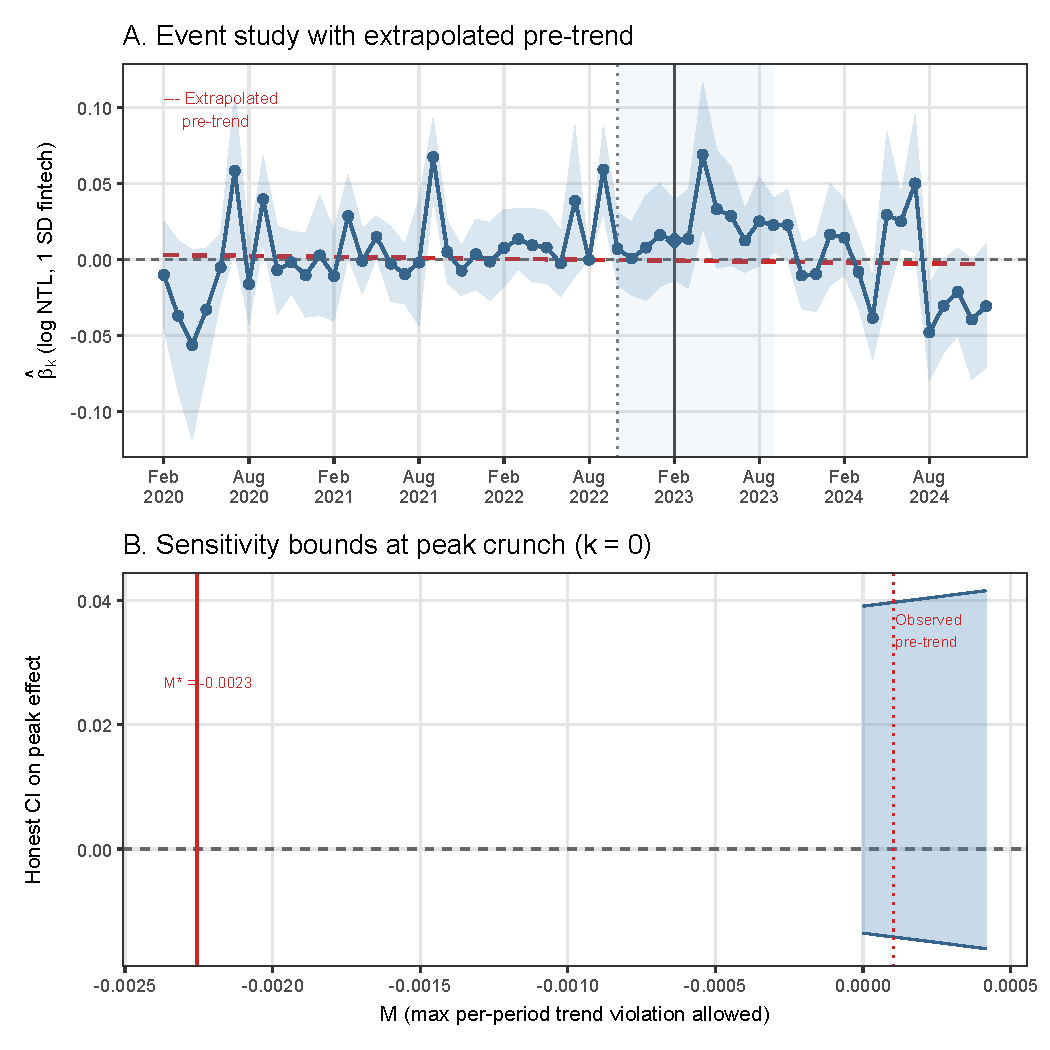
\includegraphics[width=\textwidth]{figures/fig_pretrend_sensitivity.pdf}
\caption{Pre-Trend Sensitivity Analysis}
\label{afig:pretrend_sensitivity}
\floatfoot{%
  \textit{Notes:} Panel A plots the \NTL{} event-study coefficients with the
  extrapolated pre-period trend line (dashed red). Panel B shows how the honest
  confidence interval on the peak-crunch coefficient evolves as the allowed
  per-period trend violation $M$ increases. The solid vertical line marks
  $M^* = 0.00226$, the violation required to make the lower bound touch zero.
  The dotted line marks the observed pre-period gradient $M_{\text{obs}} = 0.0001$.
  See Appendix~Table~\ref{atab:pretrend_sensitivity} for full details.
}
\end{figure}

\clearpage

% ── State trend robustness ────────────────────────────────────────────────────
\begin{figure}[H]
\centering
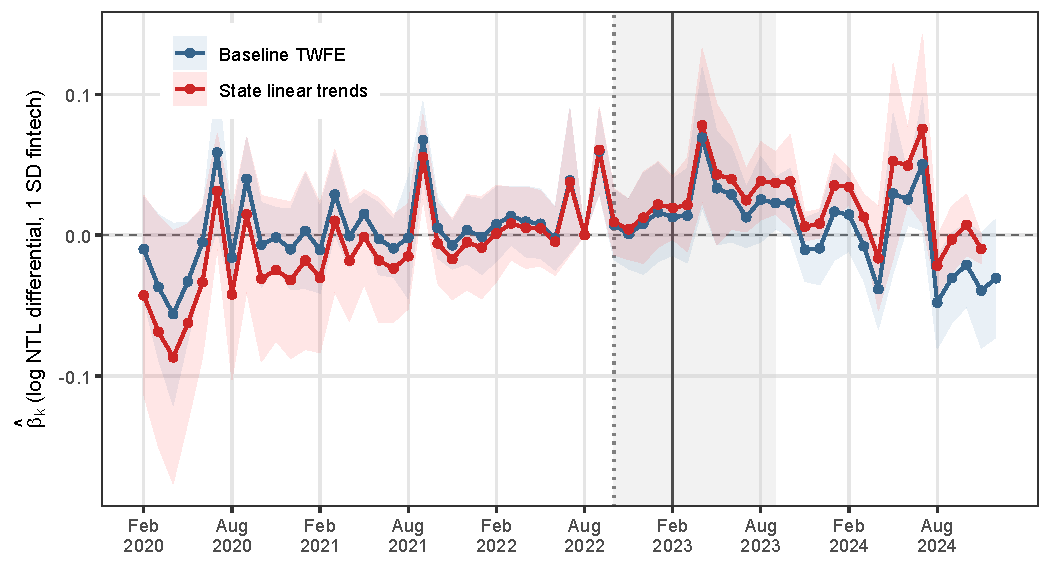
\includegraphics[width=\textwidth]{figures/fig_eventstudy_trend.pdf}
\caption{NTL Event Study: Baseline vs.\ State-Specific Linear Trend Robustness}
\label{afig:eventstudy_trend}
\floatfoot{%
  \textit{Notes:} Both lines plot round-by-round coefficients on
  $\textit{Fintech}_s \times \mathbf{1}[t=k]$ from a regression of
  $\ln(\NTL_{lt}+1)$ on state and month-year fixed effects, for baseline
  \textsc{twfe} (blue) and a specification that adds a state-specific linear
  time trend (red, dashed). The pre-period gradient is near zero in both
  specifications, validating the parallel-trends assumption. The
  trend-adjusted model shows attenuated post-announcement coefficients,
  reflecting the well-known sensitivity of state-trend specifications when
  the trend is estimated over a sample window that includes the shock period.
  Standard errors clustered at the state level.
}
\end{figure}

\clearpage

% ── Inference robustness ─────────────────────────────────────────────────────
\begin{table}[H]
\begin{threeparttable}
\caption{Firm-Level Inference Robustness: Pairs Bootstrap and Randomization Inference}
\label{atab:inference_robustness}
\small
\begin{tabular}{lcccccc}
\toprule
Outcome $\times$ Round & Coef. & Asy.\ SE & $p_{\text{asy}}$ & Boot.\ SE & $p_{\text{boot}}$ & $p_{\text{RI}}$ \\
\midrule
Enterprise active $\times$ R7 (peak crunch) & 0.0171 & 0.0076 & 0.030** & 0.0089 & 0.048** & 0.085* \\
Enterprise active $\times$ R11 (medium run) & 0.0769 & 0.0192 & 0.000*** & 0.0225 & 0.004*** & 0.000*** \\
Enterprise workers $\times$ R7 (peak crunch) & 0.2940 & 0.0550 & 0.000*** & 0.0659 & 0.002*** & 0.000*** \\
\bottomrule
\end{tabular}
\begin{tablenotes}
\footnotesize
\item \textit{Notes:} Each row reports inference for a focal hypothesis from the firm-level DiD specification (equation~\ref{eq:firm}). Coefficients are from Table~\ref{tab:firm_did}. Asy.\ SE: heteroskedasticity-robust SE clustered at the state level ($G=37$). Boot.\ SE: standard deviation of the coefficient across 999 pairs-bootstrap replications (states resampled with replacement). $p_{\text{boot}}$: fraction of centred bootstrap draws exceeding the observed absolute coefficient. $p_{\text{RI}}$: two-sided randomisation-inference $p$-value from 4999 permutations of the fintech index across states. $^{***}p<0.01$, $^{**}p<0.05$, $^{*}p<0.10$.
\end{tablenotes}
\end{threeparttable}
\end{table}


\clearpage

% ── Baseline balance ─────────────────────────────────────────────────────────
\begin{table}[H]
\begin{threeparttable}
\caption{Baseline Balance: Fintech and Pre-Shock Enterprise Characteristics}
\label{atab:balance}
\small\begin{tabular}{lcccc}
\toprule
Baseline characteristic & Coef. & SE & $p$-value & $N$ \\
\midrule
Log weekly sales (R5) & -0.0317 & 0.0528 & 0.552 & 1842 \\
Enterprise workers (R5) & -0.0780 & 0.0299 & 0.013** & 1842 \\
Rural enterprise & 0.0374 & 0.0470 & 0.431 & 1842 \\
Small firm & 0.0734 & 0.0215 & 0.002*** & 1842 \\
\bottomrule
\end{tabular}
\begin{tablenotes}\footnotesize
\item \textit{Notes:} Cross-sectional OLS at Round 5 (Aug 2022) baseline. Dependent variable is the listed enterprise characteristic. Regressor is the standardised state-level fintech index ($\textit{Fintech}_s$) measured in NLPS Round 6 (October 2022, 11 days before the CBN announcement). No fixed effects; standard errors clustered at the state level. Log weekly sales and rural location are balanced across the fintech distribution. Enterprise workers and small-firm status show statistically significant associations: high-fintech states have fewer enterprise workers ($p = 0.013$) and a higher share of small firms ($p = 0.002$) at baseline. These imbalances are absorbed by enterprise fixed effects in the main specification (equation~\ref{eq:firm}), which identifies off within-enterprise changes across rounds rather than cross-sectional differences. The heterogeneity results in Section~\ref{sub:heterogeneity} explicitly examine whether effects differ by firm size.
\end{tablenotes}\end{threeparttable}\end{table}


% ── Attrition test ────────────────────────────────────────────────────────────
\begin{table}[H]
\begin{threeparttable}
\caption{Attrition Test: Pre-Baseline Household Dropout and Fintech}
\label{atab:attrition}
\small\begin{tabular}{lcc}
\toprule
 & Coef. on Fintech & $p$-value \\
\midrule
Dropped from R3 to R5 baseline & -0.0340 & 0.203 \\
\bottomrule
\end{tabular}
\begin{tablenotes}\footnotesize
\item \textit{Notes:} Dependent variable = 1 if a household present in NLPS Round 3 (approx.\ Aug 2021) is absent from the Round 5 (Aug 2022) active enterprise sample. Regressor is the standardised state fintech index. A coefficient close to zero confirms that pre-baseline attrition is uncorrelated with the treatment variable.
\end{tablenotes}\end{threeparttable}\end{table}


\clearpage

% ── Sales null decomposition ──────────────────────────────────────────────────
\begin{table}[H]
\begin{threeparttable}
\caption{Survivor Selection and the Sales Null: Pre-Shock Sales by Fintech Tercile}
\label{atab:sales_decomp}
\small\begin{tabular}{lcccc}
\toprule
Fintech group & Survived to R7 & Exited by R7 & Difference & $N$ (surv/exit) \\
\midrule
Low fintech & 10.806 & 10.645 & 0.162 & 519 / 115 \\
Mid fintech & 10.594 & 10.928 & -0.334 & 508 / 133 \\
High fintech & 10.556 & 11.031 & -0.475 & 487 / 80 \\
\midrule
Interaction coef.\ (survived $\times$ fintech): & \multicolumn{3}{c}{-0.1699} & \\
$p$-value: & \multicolumn{3}{c}{0.131} & \\
\bottomrule
\end{tabular}
\begin{tablenotes}\footnotesize
\item \textit{Notes:} Mean log weekly sales at Round 5 (Aug 2022 pre-shock baseline) for enterprises that survived to R7 vs.\ those that had exited, by fintech tercile. If the log-sales null result at R7 reflects positive survivor selection in low-fintech states, the survival premium (survived minus exited) should be \emph{larger} in the Low fintech group. The interaction coefficient from OLS of R5 sales on survival status interacted with the continuous fintech index tests this formally; a negative coefficient would confirm stronger positive selection in low-fintech states. Standard errors clustered at the state level.
\end{tablenotes}\end{threeparttable}\end{table}


\clearpage

% ── Additional household outcomes ─────────────────────────────────────────────
\begin{table}[H]
\caption{Additional Household Outcomes: Wage Employment and Food Insecurity at Peak}
\label{tab:additional_outcomes}

\begingroup
\centering
\begin{tabular}{lccccc}
   \tabularnewline \midrule \midrule
    & Employed & \multicolumn{2}{c}{Food insecure} & Food worry & Food runout \\ 
   Dependent Variables: & employed & \multicolumn{2}{c}{food\_insecure} & food\_worry & food\_runout\\
   Model:                             & (1)             & (2)         & (3)         & (4)           & (5)\\  
   \midrule
   \emph{Variables}\\
   Fintech $\times$ R11 (medium run)  & -0.0423$^{***}$ &             &             &               &   \\   
                                      & (0.0145)        &             &             &               &   \\   
   Fintech index (std.)               &                 & -0.0083     & -0.0111     & -0.0308$^{*}$ & -0.0164\\   
                                      &                 & (0.0143)    & (0.0152)    & (0.0159)      & (0.0152)\\   
   Sample                             & Panel R5--R11   & R7 peak     & R7 peak     & R7 peak       & R7 peak\\  
   Household FE                       & \checkmark      & ---         & ---         & ---           & ---\\  
   Zone FE                            & ---             & \checkmark  & \checkmark  & \checkmark    & \checkmark\\   
   Round FE                           & \checkmark      & ---         & ---         & ---           & ---\\  
   Rural ctrl.                        & No              & No          & Yes         & Yes           & Yes\\  
   \midrule
   \emph{Fixed-effects}\\
   hh\_f                              & Yes             &             &             &               & \\  
   round                              & Yes             &             &             &               & \\  
   zone\_f                            &                 & Yes         & Yes         & Yes           & Yes\\  
   \midrule
   \emph{Fit statistics}\\
   Observations                       & 4,658           & 1,138       & 1,138       & 1,138         & 1,138\\  
   R$^2$                              & 0.63024         & 0.01475     & 0.01611     & 0.01833       & 0.02050\\  
   Within R$^2$                       & 0.00717         & 0.00015     & 0.00154     & 0.00328       & 0.00258\\  
   \midrule \midrule
   \multicolumn{6}{l}{\emph{Clustered (state\_f) standard-errors in parentheses}}\\
   \multicolumn{6}{l}{\emph{Signif. Codes: ***: 0.01, **: 0.05, *: 0.1}}\\
\end{tabular}
 
\par \raggedright 
Col (1): household wage-employment DiD (R5 Aug 2022 to R11 Apr 2024) with household FE. The negative coefficient indicates high-fintech states saw larger declines in formal wage employment, consistent with a composition shift toward self-employment in surviving enterprises (documented in Table~\ref{tab:firm_did}). Cols (2)--(5): food insecurity cross-section at R7 (peak crunch, Feb 2023). Treatment is state-level fintech index; zone FE (6 zones) absorb broad regional differences; state FE cannot be included as they are collinear with state-level treatment. Food insecure = 1 if household worried about or ran out of food in past month (FIES items). Cross-sections are descriptive; no household pre-period baseline is available. Standard errors clustered at the state level.
\par\endgroup



\end{table}

\clearpage

% ── IV first stage and leapfrog ───────────────────────────────────────────────
\begin{table}[H]
\caption{IV First Stage: Road Distance and Terrain Ruggedness}
\label{atab:iv_firststage}

\begingroup
\centering
\begin{tabular}{lcc}
   \tabularnewline \midrule \midrule
                                & (1)      & (2) \\   
   Dependent Variable: & \multicolumn{2}{c}{fintech\_std}\\
   Model:                       & (1)      & (2)\\  
   \midrule
   \emph{Variables}\\
   Constant                     & -0.9895  & -0.5092\\   
                                & (1.009)  & (1.014)\\   
   Log road dist.\ to hub (km)  & 0.2016   & 0.0960\\   
                                & (0.2027) & (0.2052)\\   
   Terrain ruggedness (std.)    &          & 0.4295$^{*}$\\   
                                &          & (0.2390)\\   
   \midrule
   \emph{Fit statistics}\\
   Observations                 & 37       & 37\\  
   R$^2$                        & 0.02749  & 0.11183\\  
   Adjusted R$^2$               & -0.00029 & 0.05958\\  
   \midrule \midrule
   \multicolumn{3}{l}{\emph{IID standard-errors in parentheses}}\\
   \multicolumn{3}{l}{\emph{Signif. Codes: ***: 0.01, **: 0.05, *: 0.1}}\\
\end{tabular}
 
\par \raggedright 
Cross-sectional OLS. Dependent variable: standardised fintech index (state level, NLPS Round 6). Road distance is the log km from each state centroid to the nearest qualifying financial hub. TRI is the mean terrain ruggedness index. Both instruments fail the relevance condition ($F<10$) and exhibit the wrong sign (states farther from hubs have higher fintech, reflecting the leapfrog dynamic documented in Appendix Table~\ref{atab:leapfrog}). Heteroskedasticity-robust standard errors.
\par\endgroup



\end{table}

\clearpage

\begin{table}[H]
\begin{threeparttable}
\caption{The Leapfrog Dynamic: Financial Exclusion (2014) and Fintech Adoption (2022)}
\label{atab:leapfrog}
\small\begin{tabular}{lccc}
\toprule
Geopolitical zone & Unbanked (2014, \%) & Fintech index (2022, \%) & States ($N$) \\
\midrule
3 & 38.3 & 30.3 & 7 \\
1 & 32.2 & 30.1 & 7 \\
4 & 30.7 & 25.6 & 5 \\
5 & 30.6 & 24.6 & 6 \\
6 & 21.1 & 24.4 & 6 \\
2 & 19.4 & 31.3 & 6 \\
\midrule
Pearson $r$ & \multicolumn{3}{c}{0.126} \\
\bottomrule
\end{tabular}
\begin{tablenotes}\footnotesize
\item \textit{Notes:} Zone-level means. Unbanked (2014) is the share of WBES 2014 firms without a bank account (proxy for initial financial exclusion). Fintech index (2022) is the mean state-level digital payment penetration from NLPS Round 6 (October 2022). The weak, near-zero correlation ($r=0.13$) between 2014 exclusion and 2022 fintech adoption reflects the leapfrog dynamic: zones that were most financially excluded in 2014 had the strongest incentive to adopt mobile money between 2014 and 2022, invalidating road distance to financial hubs as an instrument for fintech adoption. This explains the wrong-sign first-stage coefficient in Appendix Table~\ref{atab:iv_firststage}.
\end{tablenotes}\end{threeparttable}\end{table}


\clearpage


\begingroup
\centering
\begin{tabular}{lcc}
   \tabularnewline \midrule \midrule
   Dependent Variable: & \multicolumn{2}{c}{fintech\_std}\\
   Model:                                    & (1)                     & (2)\\  
   \midrule
   \emph{Variables}\\
   Constant                                  & $-2.75\times 10^{-17}$  & -1.399\\   
                                             & (0.1661)                & (1.031)\\   
   R1 digital payment index (std., Aug 2021) & 0.1877                  & 0.2530\\   
                                             & (0.1684)                & (0.1729)\\   
   Log road dist.\ to hub                    &                         & 0.2850\\   
                                             &                         & (0.2075)\\   
   \midrule
   \emph{Fit statistics}\\
   Observations                              & 37                      & 37\\  
   R$^2$                                     & 0.03431                 & 0.08511\\  
   Adjusted R$^2$                            & 0.00672                 & 0.03129\\  
   \midrule \midrule
   \multicolumn{3}{l}{\emph{IID standard-errors in parentheses}}\\
   \multicolumn{3}{l}{\emph{Signif. Codes: ***: 0.01, **: 0.05, *: 0.1}}\\
\end{tabular}
 
\par \raggedright 
Cross-sectional OLS. Dependent variable: standardised R6 fintech index (Oct 2022). Instrument: state-level share of households using any digital payment in NLPS Round 1 (August 2021, 14 months before the CBN announcement). This predetermines the fintech infrastructure readiness before the 2022-specific adoption dynamics. Heteroskedasticity-robust SEs.
\par\endgroup




\clearpage

% ── Alternative treatment index definitions ───────────────────────────────────
\begin{table}[H]
\caption{Robustness: Alternative Treatment Definitions}
\label{atab:alt_treatment}

\begingroup
\centering
\begin{tabular}{lcccc}
   \tabularnewline \midrule \midrule
                                  & Baseline (4-svc) & All 8 services & Payments only\\(mobile+USSD)   & Bank acct only \\   
   Dependent Variable: & \multicolumn{4}{c}{ln\_ntl\_mean}\\
   Model:                         & (1)              & (2)            & (3)                            & (4)\\  
   \midrule
   \emph{Variables}\\
   Fintech (4-svc) $\times$ Peak  & 0.0189           &                &                                &   \\   
                                  & (0.0154)         &                &                                &   \\   
   All-8 $\times$ Peak            &                  & 0.0315         &                                &   \\   
                                  &                  & (0.0248)       &                                &   \\   
   Payments-only $\times$ Peak    &                  &                & -0.0020                        &   \\   
                                  &                  &                & (0.0128)                       &   \\   
   Bank acct $\times$ Peak        &                  &                &                                & 0.0256\\   
                                  &                  &                &                                & (0.0153)\\   
   \midrule
   \emph{Fixed-effects}\\
   state                          & Yes              & Yes            & Yes                            & Yes\\  
   date\_fct                      & Yes              & Yes            & Yes                            & Yes\\  
   \midrule
   \emph{Fit statistics}\\
   Observations                   & 2,664            & 2,664          & 2,664                          & 2,664\\  
   R$^2$                          & 0.93148          & 0.93147        & 0.93083                        & 0.93126\\  
   Within R$^2$                   & 0.01016          & 0.01001        & 0.00086                        & 0.00705\\  
   \midrule \midrule
   \multicolumn{5}{l}{\emph{Clustered (state) standard-errors in parentheses}}\\
   \multicolumn{5}{l}{\emph{Signif. Codes: ***: 0.01, **: 0.05, *: 0.1}}\\
\end{tabular}
 
\par \raggedright 
Peak crunch period coefficient only. All specifications include state and month-year FEs. Column (3) uses only mobile money and USSD/mobile banking (the two categories most directly substitutable for cash during the crunch). Clustered SEs at the state level.
\par\endgroup



\end{table}

\clearpage

% Summary statistics appear in Table~\ref{tab:summary} of the main text (Section~\ref{sec:data}).
